\chapter{Herramientas para trabajar con Android} \label{ch:androidTools}

Para desarrollar una aplicación, debemos de contar con las herramientas necesarias para hacerlo, y esto no es una excepción cuando trabajamos con Android. Las herramientas más habituales son:

\begin{enumerate}
  \item Android \acrfull{SDK}: Es un conjunto de herramientas para el desarrollo de aplicaciones en Android. Comprende un depurador de código, biblioteca, emulador de terminales, documentación, ejemplos y tutoriales.
  \item \acrfull{ADB}: Aplicación incluida dentro del \gls{SDK} compuesta por tres componentes: un cliente y un servidor que se ejecutan en la máquina de desarrollo, y un daemon que se ejecuta en el termina. Esta aplicación nos permite la comunicación ya sea a través de línea de comandos (comando adb) o a través de una interfaz gráfica (consola de depuración de Google Chrome) con los dispositivos Android conectados vía \gls{USB} o que están siendo emulados.
  \item \acrfull{AVD}: Herramienta para emular dispositivos Android basada en \emph{qemu}\footnote{\url{http://www.qemu-project.org/}}
  \item Android Studio: Se trata de un \gls{IDE} basado en ItelliJ y que vino a sustituir a Eclipse como \gls{IDE} oficial a la hora de programar aplicaciones para Android.
\end{enumerate}

Para instalar estas herramientas tenemos dos opciones. Instalar tanto Android Studio como Android SDK, o descargarnos las herramientas que conforman Android SDK en caso de querer trabajar con un IDE diferente. En nuestro caso, vamos a instalar solamente Android SDK, ya que para trabajar con tecnologías web existen alternativas mejores que Android Studio.

\section{Instalación de Android SDK}

Android SDK es un conjunto de herramientas que podemos descargar en forma de fichero comprimido, por lo que más que instalar, lo que haremos será descargarnos este fichero y descomprimirlo en nuestro ordenador. Antes de ver como poder descargárnoslo y explicar algunos de sus componentes y como usarlos, vamos a explicar como instalar el \glsfirst{JDK}, software necesario para poder utilizar las herramientas de Android.

\begin{enumerate}
  \item Accedemos a la página de descarga de Java, propiedad de Oracle, \url{http://www.oracle.com/technetwork/java/javase/downloads/index.html}, donde veremos la opción de para descargarnos el \gls{JDK}.
  \item Deberemos aceptar los términos de uso y elegir la versión que necesitamos antes de empezar con la descarga.
  \begin{figure}[H]
\centering
    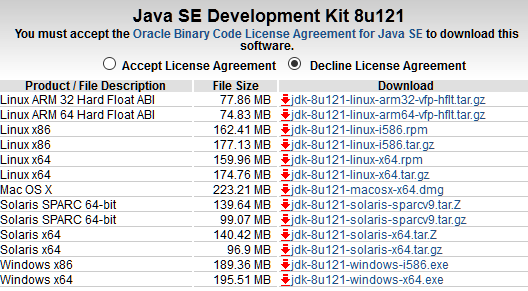
\includegraphics[width=0.8\textwidth]{Figures/anexo/android_tools/jdk_download}
    \caption{\glsfirst{JDK} está disponible para diferentes sistemas operativos y arquitecturas.}
  \end{figure}
  \item Es importante durante la instalación ver la localización donde se va a realizar, ya que puede ser necesario indicar esta ruta de instalación por si nos la requiere el SDK de Android.
  \begin{figure}[H]
\centering
    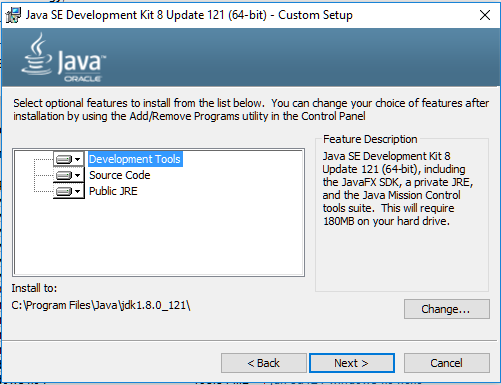
\includegraphics[width=0.8\textwidth]{Figures/anexo/android_tools/jdk_custom_setup_1}
    \caption{Durante la instalación podremos cambiar la ruta de instalación del \gls{JDK}, aunque se recomienda no modificarla si no es estrictamente necesario.}
  \end{figure}
  \item  Lo mismo ocurre con la ruta de instalación de \glsfirst{JRE}.
\end{enumerate}

Si todo ha ido bien, podremos ejecutar el comando de Java desde consola.

\begin{figure}[H]
\centering
  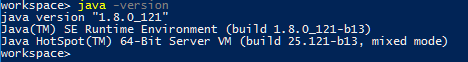
\includegraphics[width=0.8\textwidth]{Figures/anexo/android_tools/jdk_check}
  \caption{Podemos comprobar desde la consola la versión del \gls{JDK} que tenemos instalada.}
\end{figure}

Con el \gls{JDK} ya disponible en nuestro equipo, podemos descargarnos el \gls{SDK} de Android desde la página de desarrolladores que ofrece Google, \url{https://developer.android.com/studio/index.html#downloads}. En esta página podremos encontrar el instalador de Android Studio (opción mas destacada) y el \gls{SDK} de manera individual. De ambos existen versiones para diferentes sistemas.

\begin{figure}[H]
\centering
  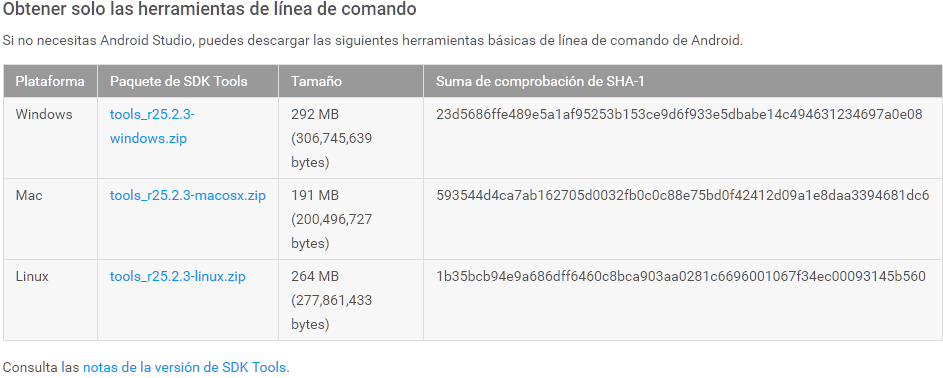
\includegraphics[width=0.8\textwidth]{Figures/anexo/android_tools/sdk_download}
  \caption{Aunque la opción está un poco ``escondida'', podemos descargarnos el \gls{SDK} de Android sin necesidad de instalar Android Studio.}
\end{figure}

Cuando se haya completado la descarga, podremos descomprimir el fichero en el directorio que queramos y poder ver los componentes que forman Android \gls{SDK}.

\begin{figure}[H]
\centering
  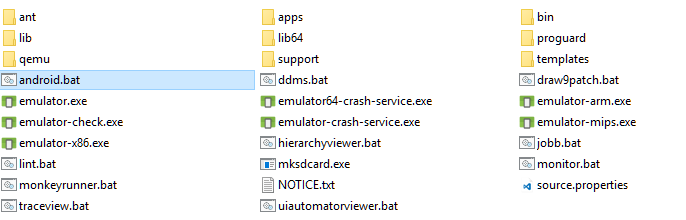
\includegraphics[width=0.8\textwidth]{Figures/anexo/android_tools/sdk_uncompressed}
  \caption{Ficheros que se encuentran dentro del paquete comprimido.}
\end{figure}

\section{Android SDK Manager}\label{sec:SDKManager}

El paquete de Android \gle{SDK} cuenta \emph{Android SDK Manager}, que nos permite instalar las herramientas que ofrece el SDK, las plataformas y  otros componentes de manera independiente. Una vez iniciado veremos una ventana como la siguiente:

\begin{figure}[H]
\centering
  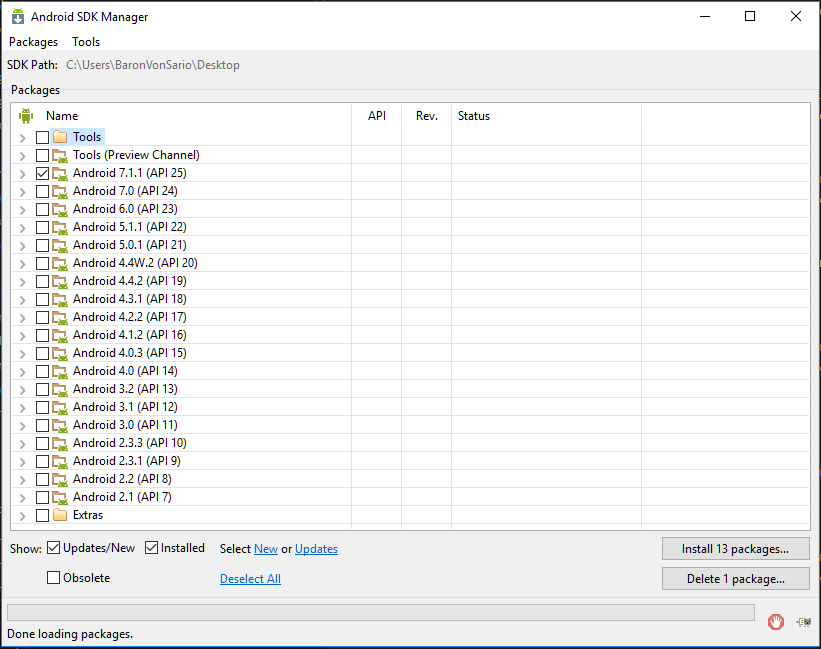
\includegraphics[width=0.8\textwidth]{Figures/anexo/android_tools/sdk_manager}
  \caption{Android SDK Manager nos permite instalar los diferentes componentes de Android SDK por separado.}
\end{figure}

Los componentes aparecen agrupados en diferentes grupos:

\paragraph{Tools} Aquí se encuentran varias herramientas indispensables para poder crear una aplicación para Android. Es recomendable instalar la última versión de aquellas que aparezcan. Los paquetes herramientas que nos encontramos son \textbf{Android SDK tools}, que contiene elementos como el emulador, \textbf{Android SDK Platform-tools}, donde se incluye \gls{ADB} y \textbf{Android SDK Build-tools}, con las herramientas que compilan y generan la aplicación.

\paragraph{Android SDK Platform} Diferentes versiones de la plataforma Android. Al menos tendremos que tener una de ellas disponible, que bien puede ser la última, lo cuál es lo más recomendable, o bien una anterior, según los requisitos del desarrollo. Aquí también se encuentran las imágenes del sistema que podremos ejecutar en el emulador.

\paragraph{Extras} Software que no se engloba en ninguno de los otros grupos pero que pueden ser de utilidad durante el desarrollo de nuestro proyecto. Aquí se podemos encontrarnos con los drivers \textbf{Google USB}, que dependiendo del dispositivo que tengamos, necesitaremos instalar para poder conectarlo a nuestro \gls{PC}; el \textbf{repositorio de Google}, con diferentes bibliotecas; o \textbf{Google Play services}.

\section{Android Virtual Device}\label{sec:AVD}

Llamamos \acrfull{AVD}\footnote{\url{https://developer.android.com/studio/run/managing-avds.html}} a la definición de características de un dispositivo Android, ya sea un teléfono, una tablet, un smartwatch, \ldots. Entre otras propiedades, se encuentra el hardware del dispositivo, la imagen del sistema o el espacio de almacenamiento asociado. Los \gls{AVD} pueden ser emulados usando \nameref{sec:AndroidEmulator}.

Para gestionar nuestros \glspl{AVD} disponemos de un manager al que podemos acceder desde el \nameref{sec:SDKManager}.

\begin{figure}[H]
\centering
  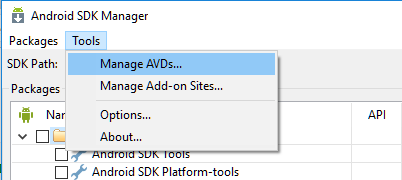
\includegraphics[width=0.8\textwidth]{Figures/anexo/android_tools/avd_open_manager}
  \caption{Desde el propio manager de Android SDK podremos abrir el manager de avds.}
\end{figure}

Esto nos abre una ventana como la siguiente en la que podemos ver dos pestañas. En una aparecerá una lista con los \glspl{AVD} disponibles, en la otra, una lista de definiciones de dispositivos.

\begin{figure}[htbp]
\centering
\subfigure[Lista de AVDs]{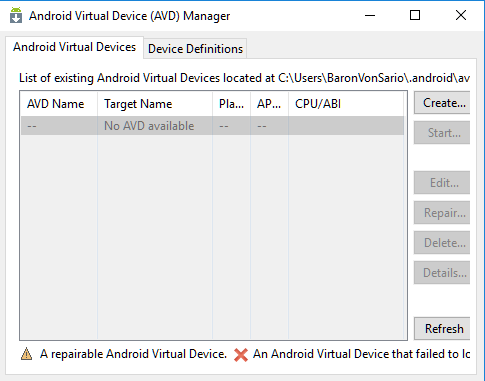
\includegraphics[width=0.45\textwidth]{Figures/anexo/android_tools/avd_manager_avds_list}}\hspace{0.05\textwidth}
\rulesep
\subfigure[Lista de definiciones de dispositivos]{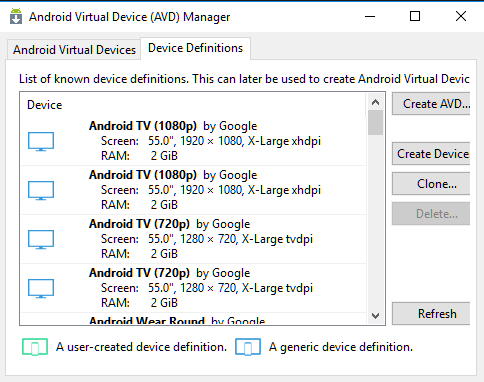
\includegraphics[width=0.45\textwidth]{Figures/anexo/android_tools/avd_manager_definitions_list}}
\caption{AVDs Manager.}
\end{figure}

En el listado de dispositivos podemos ver algunos que vienen por defecto, entre los que encontramos terminales de la familia Nexus, Android TV, smartwatchs y tablets. Con estos dispositivos debería ser más que suficiente, pero si queremos, podemos crear los nuestros propios desde cero, o clonando alguno de los ya existentes, y así poder personalizar al gusto las características del hardware.

\begin{figure}[H]
\centering
  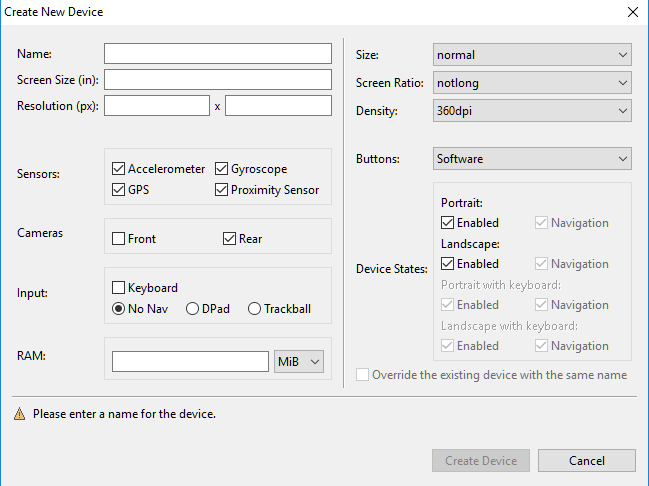
\includegraphics[width=0.8\textwidth]{Figures/anexo/android_tools/avd_manager_definitions_create}
  \caption{A la hora de crear un nuevo dispositivo, podemos configurar varias características de su hardware.}
\end{figure}

Por otro lado, la lista de \glspl{AVD} se encuentra vacía ya que no viene ninguna configuración establecida por defecto. Para crear la nuestra y poder emularla, pulsamos el botón \textbf{Create AVD}. Nos abrirá una ventana donde podremos configurar nuestro \gls{AVD}.

\begin{figure}[H]
\centering
  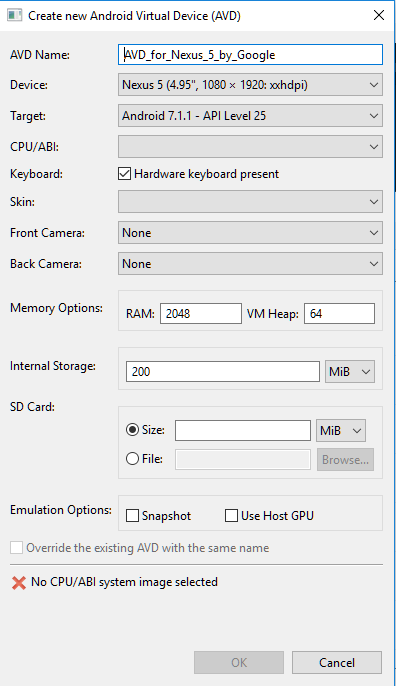
\includegraphics[width=0.6\textwidth]{Figures/anexo/android_tools/avd_manager_avds_create}
  \caption{Vista con la que podemos crear nuestro \gls{AVD}.}
\end{figure}

Los campos que debemos rellenar en este paso son:

\begin{enumerate}
  \item AVD Name: Nombre con el que identificar nuestro \gls{AVD}, tanto dentro del manager, como fuera. Este nombre será el que se utilice para identificar el emulador en herramientas externas, como Ionic CLI cuando se usa la opción \emph{emulate}.
  \item Device: Definición del dispositivo que queremos que se use. En esta lista aparecerán los dispositivos por defecto y los que hayamos creado nosotros.
  \item Target: Versión de la plataforma Android que usará. Solo aparecerán aquellas que se hayan descargado previamente desde el \gls{SDK} manager.
  \item CPU/ABI: Imagen del sistema. También tendrá que ser descargado con anterioridad junto con la versión de la plataforma desde el \gls{SDK} manager.
  \item Keyboard: Si habilitamos esta opción, el emulador entenderá que el dispositivo dispone de un teclado físico por lo que no se mostrará el teclado virtual.
  \item Skin: Aspecto que debe utilizar el dispositivo y que definirá el tamaño con el que se verán los elementos de la aplicación, como los botones.
  \item Front/Back Camera: Cámaras que tendrá el dispositivo. En caso de disponer, la imagen puede ser emulada, o utilizar una webcam conectada a nuestra máquina.
  \item Memory Option: Memoria RAM que utilizará el emulador. Debemos de configurar esta cantidad teniendo en cuenta la memoria RAM disponible en la máquina en la cual vayamos a ejecutar el emulador.
  \item Internal Storage y SD Card: Capacidad de almacenamiento que tendrá el dispositivo emulado y que podremos definir por separado según se trate del propio almacenamiento del sistema, o corresponde a una memoria extraíble.
  \item Emulation Option: Estas opciones tienen que ver con el rendimiento del emulador. La opción \emph{Snapshot} crea una ``copia'' del sistema emulado en la memoria RAM lo que acelera un posible reinicio de la aplicación. La opción \emph{Use Host GPU} como se puede uno imaginar, hace que el emulador haga uso de la tarjeta gráfica de la máquina que lo ejecuta, acelerando las operaciones relacionadas con la visualización.
\end{enumerate}

\section{Android Emulator}\label{sec:AndroidEmulator}

El emulador de Android\footnote{\url{https://developer.android.com/studio/run/emulator.html}} que ofrece Android \gls{SDK}, basado en \textbf{qemu}\footnote{\url{http://www.qemu-project.org/}}, nos permite emular nuestros \glspl{AVD} y ejecutar dentro las aplicaciones Android que desarrollamos.

El emulador nos permite además, simular diferentes características de las que dispone el dispositivo real y con los que no contamos en la máquina de desarrollo. Un ejemplo son las cámaras con las que cuentan la mayoría de dispositivos, y que como vimos en la creación de \glspl{AVD}, podemos simular.

\begin{figure}[H]
\centering
  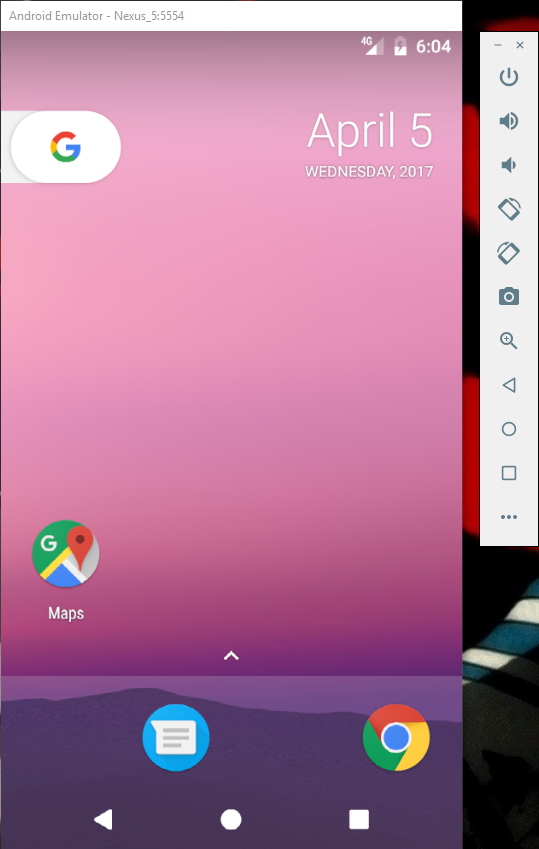
\includegraphics[width=0.45\textwidth]{Figures/anexo/android_tools/emulator}
  \caption{Emulador de Android, con la pantalla a la izquierda y la botonera a la derecha.}
\end{figure}

Al ejecutar el emulador nos aparece por un lado una ventana que simula la pantalla del dispositivo, y por otro una barra vertical con botones. La pantalla actua como la de un dispositivo real en la que el puntero del ratón hace de dedo. El gesto de pellizco, en el cual se usan dos dedos, se puede simular pulsando la tecla Ctrl o Command (⌘). Además, si arrastramos nuestra \gls{APK} sobre esta pantalla, el emulador instalará la aplicación en el simulador; en caso de arrastrar otro tipo de archivos, este se almacenará como un fichero dentro del sistema emulado.

En la barra vertical contamos con diferentes funciones típicas de un terminal móvil y que se suelen reflejar mediante un botón físico o software en los terminales reales. Ejemplo de esto es el botón de apagado, los de volumen, la botonera inferior característica de Android (que según el modelo de dispositivo, son implementados vía software o mediante botones físicos), \ldots.

Al final de la barra vertical se encuentra un botón con el cual podremos abrir los controles extendidos.

\begin{figure}[H]
\centering
  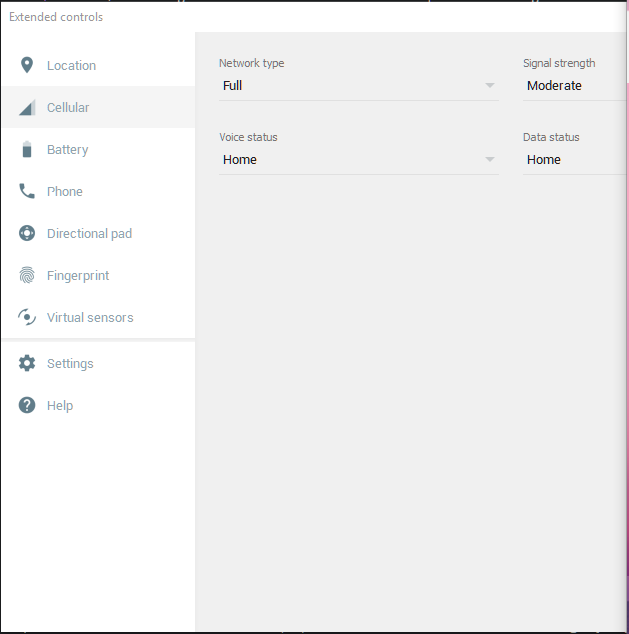
\includegraphics[width=0.8\textwidth]{Figures/anexo/android_tools/emulator_extended_controls}
  \caption{Ventana de controles extendidos del emulador.}
\end{figure}

Desde esta ventana podremos simular diferentes sensores, llamadas, estado de la batería, \ldots.
